
\def\colegio{Colegio Latinoamericano de Integración}
\def\titulo{Guía}
\def\subtitulo{Ecuaciones}
\documentclass[options]{plantilla-material-v1}

\begin{document}
\section{Operatoria algebraica}

Reduce las siguientes expresiones algebraicas.
\begin{ejercicios}[resume](1)
  \ejercicio $3x +6y +2x -4y$
  \ejercicio $6m -17n +8n +7m -2n$
  \ejercicio $2x +6y +3x^2 +5x +5x^2$
  \ejercicio! $4a -2ab^3 +3b +5a +8ab^3$
  \ejercicio $2ab + 2b -(4ab+5b)$
  \ejercicio $3b + 3xy -(-6b+8xy)$
\end{ejercicios}

Considera las siguientes igualdades y luego calcula.
\figuraTriple{$A=m+n$}{$B=2m-n$}{$C=4m-3n$}
\begin{ejercicios}[resume](2)
  \ejercicio $A+B$
  \ejercicio $A+B+C$
  \ejercicio $A-B$
  \ejercicio $B-A$
  \ejercicio $A-(B+C)$
  \ejercicio $B-(A+C)$
\end{ejercicios}

Desarrolla los siguientes productos.
\begin{ejercicios}[resume](1)
  \ejercicio $3\cdot(a+d)$
  \ejercicio $b\cdot(3d-f)$
  \ejercicio $2b\cdot(l+3t-8b)$
  \ejercicio $5t\cdot(8d-2r+d^5)$
  \ejercicio $(2+f)\cdot(g+3h)$
  \ejercicio $(r+5t)\cdot(k-g)$
  \ejercicio $(m-n)\cdot(q-p+1)$
  \ejercicio $t^2\cdot(5d-2l+11+t^2)$
\end{ejercicios}

Considera las siguientes igualdades y luego calcula.
\figuraTriple{$A=m+1$}{$B=2m-3$}{$C=4m-3n$}
\begin{ejercicios}[resume](2)
  \ejercicio $2A$
  \ejercicio $5B$
  \ejercicio $A\cdot B$
  \ejercicio $B\cdot C$
  \ejercicio $2\cdot(B+C)$
  \ejercicio $6\cdot(A-C)$
\end{ejercicios}

Resuelve las siguientes multiplicaciones de expresiones algebraicas. Luego, reduce los
términos semejantes.

\begin{ejercicios}[resume](1)
  \ejercicio $5x\cdot8x$
  \ejercicio $(8-4y^2+3x^2)\cdot 10xy$
  \ejercicio $(-x^2+2x)\cdot(5x-0.5x^2)$
  \ejercicio $(11mn+3m^2n)\cdot(-4mn^2-mn+0.25)$
  \ejercicio $\left(\dfrac{1}{2}xy+\dfrac{1}{4}\right)\cdot
    \left(\dfrac{3}{4}x^2-\dfrac{1}{2}xy\right)$
  \ejercicio $\left(\dfrac{1}{5}a-\dfrac{3}{2}b-2\right)\cdot
    \left(-2a-\dfrac{1}{7}b+1\right)$
  \ejercicio $\left(\dfrac{2}{3}x^3y-\dfrac{4}{7}xy\right)\cdot
    \left(\dfrac{5}{8}xy-\dfrac{6}{5}x^2y\right)$
  \ejercicio $(-4ab^2+3a^2b^2-5ab^2-2)\cdot(-6ab+5)$
\end{ejercicios}

Determina una expresión algebraica reducida para el área y perimetro de las siguientes
figuras.
\begin{ejercicios}[resume](1)
  \ejercicio
  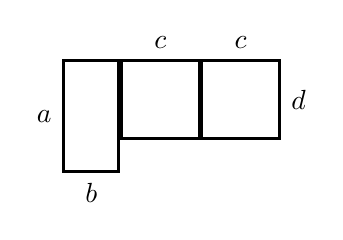
\begin{tikzpicture}[baseline=(current bounding box.north),line width=1pt]
    \node[draw,shape=rectangle,inner ysep=20,inner xsep=10] (R) {};
    \node[draw,shape=rectangle,inner sep=14,anchor=north west] (Q) at (R.north east) {};
    \node[draw,shape=rectangle,inner sep=14,anchor=north west] (QQ) at (Q.north east) {};
    \node[left] at (R.west) {$a$};
    \node[below] at (R.south) {$b$};
    \node[above] at (Q.north) {$c$};
    \node[above] at (QQ.north) {$c$};
    \node[right] at (QQ.east) {$d$};
  \end{tikzpicture}
  \ejercicio
   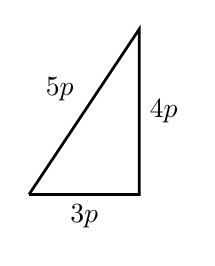
\begin{tikzpicture}[scale=0.7,baseline=(current bounding box.north),line width=1pt]
      \draw (0,0) -- (2,0) node[midway,below] {$3p$} --([turn]90:3) node[midway,right] {$4p$} -- (0,0)
        node[midway,above left] {$5p$};
   \end{tikzpicture}
\end{ejercicios}

\section{Solucionar para una incógnita}
\NewDocumentCommand{\incognita}{}{
  \tcbox[colback=black!60, colframe=black!60, coltext=white, on line, boxsep=0pt, left=2pt, right=2pt, top=2pt, bottom=2pt,width=1cm]{\bfseries ?}
}
En cada caso, determine el término que falta para que se cumpla la igualdad.
\begin{ejercicios}[resume](1)
  \ejercicio $6m+4n+\incognita + 6n = 17m +10n$
  \ejercicio $3ab + 6b + \incognita - 10b = 5ab - 4b$
  \ejercicio $4x+8y+\incognita + 5x + 7x^2 = 8x +8y +16x^2$
  \ejercicio $7a -8ab^3 +6b +5a +9ab^3 = \incognita + 6b + ab^3$
\end{ejercicios}

Determina la medida del lado desconocido en cada rectángulo considerando el área dada.
\begin{ejercicios}[resume](2)
  \ejercicio 
  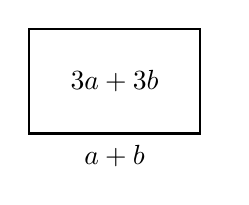
\begin{tikzpicture}[scale=0.5,baseline=(current bounding box.north),line width=1pt]
    \node[draw,shape=rectangle,name=R,inner sep=15pt] {$3a+3b$};
    \node[below] at (R.south) {$a+b$};
    \node[right] at (R.east) {\incognita}; 
  \end{tikzpicture}
  \ejercicio 
  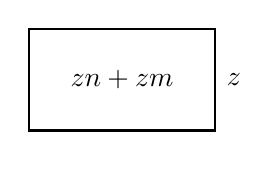
\begin{tikzpicture}[scale=0.5,baseline=(current bounding box.north),line width=1pt]
    \node[draw,shape=rectangle,name=R,inner sep=15pt] {$zn+zm$};
    \node[below] at (R.south) {\incognita};
    \node[right] at (R.east) {$z$}; 
  \end{tikzpicture}
  \ejercicio!
  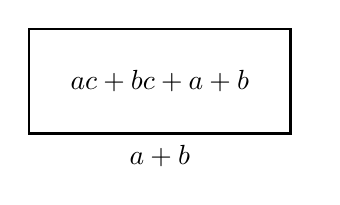
\begin{tikzpicture}[scale=0.5,baseline=(current bounding box.north),line width=1pt]
    \node[draw,shape=rectangle,name=R,inner sep=15pt] {$ac+bc+a+b$};
    \node[below] at (R.south) {$a+b$};
    \node[right] at (R.east) {\incognita}; 
  \end{tikzpicture}

\end{ejercicios}

Resuelve las siguientes ecuaciones.
\begin{ejercicios}
  \ejercicio $x+2=8$
  \ejercicio $x-5=6$
  \ejercicio $8-x=6$
  \ejercicio $2x+6=8$
  \ejercicio $-(1-x)=2x-2$
  \ejercicio $\dfrac{x}{2}-2=-6$
  \ejercicio $x+\dfrac{1}{x}=2x-\dfrac{1}{6}$
  \ejercicio $-\left(x-\dfrac{1}{6}\right)+\dfrac{1}{2}=\dfrac{1}{3}$
  \ejercicio $3x-4=-11$
  \ejercicio $3-x=3x$
  \ejercicio $4-\dfrac{x}{2}=\dfrac{18}{4}$
  \ejercicio $-x+11=-2x+6$
  \ejercicio $3(x-6)=2(9-3x)$
  \ejercicio $\dfrac{x}{2}=1-\dfrac{3x}{4}$
  \ejercicio $3x-4=6x+20$
  \ejercicio $3,5x+4=2,5x-5$
  \ejercicio $2(x+7)=3(x-1)$
  \ejercicio $\dfrac{x}{2}+\dfrac{7}{4}=\dfrac{3}{2}$
  \ejercicio $\dfrac{3x}{10}-\dfrac{6}{5}=\dfrac{3}{5}$
\end{ejercicios}

Asegúrate de reemplazar los valores obtenidos en la expresión original, para 
verificar que los valores son realmente solución de la ecuación y no realizamos
algún error de cálculo.

\begin{equation*}
  \begin{split}
    -\dfrac{1}{2}(-3x+1) +3 &= 8,5 \\
     -\dfrac{1}{2}\cdot-3x -\dfrac{1}{2}\cdot1 +3 &= 8,5 \\
     +1,5x-0,5+3 &= 8,5 +3,5 \\
     1,5x + 2,5 &= 8,5 \\
     1,5x &= 6 \\
     x &= \dfrac{6}{1,5} \\
     x &= \dfrac{60}{15} \\
     x &= 4.
  \end{split}
\end{equation*}

Reemplazando $x=4$ en la expresión original, queda que:
\begin{equation*}
  \begin{split}
    -\dfrac{1}{2}(-3\cdot4+1) +3 &= 8,5 \\
    -0,5\cdot(-12+1) + 3 &= 8,5 \\
    -0,5\cdot-11 + 3 &= 8,5 \\
    5,5 + 3 &= 8,5 \\
    8,5 &= 8,5
  \end{split}
\end{equation*}

Intenta resolver alternativamente la primera expresión usando fracciones en lugar 
de números decimales.

\section{Modelar usando ecuaciones}

Escribe una expresión algebraica que represente cada caso.
\begin{ejercicios}(1)
  \ejercicio Un número aumenta en 2.
  \ejercicio El quíntuple de un número.
  \ejercicio El sucesor del doble de un número.
  \ejercicio El triple de un número es igual al número más 8.
\end{ejercicios}

Representa cada enunciado con una ecuación.
\begin{ejercicios}(1)
  \ejercicio La suma de dos números consecutivos aumentada en 10 unidades equivale al mayor
  de ellos aumentado en 9 unidades.
  \ejercicio Un número equivale a la cuarta parte del número disminuido en 3 unidades.
  \ejercicio La tercera parte de un número disminuida en 10 unidades equivale al triple 
  del número.
  \ejercicio La suma de tres números pares consecutivos equivale a 42 unidades.
\end{ejercicios}

Plantea una ecuación para cada problema y luego resuelve.
\begin{ejercicios}(1)
  \ejercicio La producción de un evento tiene un costo de \$1.500.000 Si cada entrada
  se vende a \$10.000, ¿cuántas entradas hay que vender para obtener una ganancia de 
  \$800.000?
  \ejercicio Sofía compró $\frac{3}{4}$ kg de pan y $\frac{5}{8}$ kg de queso y gastó
  \$4.560. Si el precio de un kilogramo de pan es de \$1080, ¿cuál es el precio
  de 1 kg de queso?
  \ejercicio Tomás tiene tres cuartos de la edad de su hermana mayor. Si las 
  edades de ambos suman 35 años, ¿qué edad tiene su hermana?
  \ejercicio Si el perímetro de un rectángulo es de 96,6 cm y la medida del largo es el
  doble que la medida del ancho, ¿cuáles son sus dimensiones?
  \ejercicio Una avenida está siendo asfaltada por etapas. En la primera etapa se asfaltó
  la mitad; en la segunda, la quinta parte, y en la tercera, la cuarta parte del total.
  ¿Cuál es la longitud de la avenida si aún faltan 200 m por asfaltar?
  \ejercicio Un triángulo isósceles tiene un perímetro de $(3x+19)$ cm. Si la medida de su
  base es $(x+5)$ cm, ¿cuánto miden sus lados?
  \ejercicio Las medidas de los lados de un rectángulo se diferencian en 12 cm. Si la 
  medida del lado de menor longitud es $(2x+20)$, ¿cuál es el área y el perímetro del
  rectángulo?
  \ejercicio Un joyero regalará su colección de relojes. La mitad se la dará a su hija,
  la tercera parte del resto se la regalará a su nieta, la mitad de los que queda se lo
  entregará a su sobrino y el resto, que son cinco relojes, se los dará a su hermano.
  \begin{preguntas}
    \pregunta ¿Cuántos relojes tiene su colección?
    \pregunta ¿Cuántos relojes recibirá cada uno?
  \end{preguntas}
\end{ejercicios}

\end{document}